\chapter{Tempo discreto, malha interna da Pixhawk e atrasos}
\label{cap:discreto}

Os modelos ideais do \cref{cap:modelagem} supõem que a aceleração pedida acontece na
hora. No sistema real, (i) o controlador roda a \SI{20}{Hz}; (ii) a PX4 leva algumas
centenas de milissegundos para seguir o setpoint; (iii) a medida do alvo chega
atrasada. Este capítulo mostra como incluir os três efeitos no projeto.

\section{Amostragem e o plano $z$}
Um polo contínuo $s$ corresponde ao polo discreto $z=e^{s\Ts}$. Logo:
\begin{itemize}
  \item a estabilidade passa a ser $|z|<1$ (círculo unitário);
  \item o amortecimento vira o raio: $|z| = e^{-\zeta\omega_n \Ts}$;
  \item a frequência amortecida vira o ângulo: $\angle z = \omega_n\sqrt{1-\zeta^2}\,\Ts$.
\end{itemize}
Exemplo com $\Ts=\SI{0,05}{s}$, $\zeta=0{,}7$, $\omega_n=\SI{2,3}{rad/s}$:
$|z| = e^{-0{,}08}=0{,}923$ e $\angle z = \SI{0,082}{rad}$. Os polos ficam perto de
$z=1$, o que é normal quando a amostragem é rápida em relação à dinâmica.

\paragraph{Escolha do período.} Regra usual: $\omega_c\Ts\in[0{,}05;\ 0{,}2]$, ou seja,
10 a 30 amostras por tempo de subida. Com $\omega_c\approx 1$--\SI{3}{rad/s} e
$\Ts=\SI{0,05}{s}$, $\omega_c\Ts\approx0{,}05$--$0{,}15$, então \SI{20}{Hz} basta. Subir
para \SI{50}{Hz} quase não muda o resultado, porque o gargalo é a câmera a \SI{30}{Hz}.

\section{Métodos de discretização}
\begin{table}[H]
\centering
\begin{tabular}{@{}lll@{}}
\toprule
Método & Mapeamento & Uso \\
\midrule
ZOH (exato p/ entrada constante) & $G(z) = (1-z^{-1})\mathcal Z\{G(s)/s\}$ & planta (\code{c2d(G,Ts,'zoh')}) \\
Tustin (bilinear) & $s = \frac{2}{\Ts}\frac{z-1}{z+1}$ & controladores (\code{c2d(C,Ts,'tustin')}) \\
Euler para trás & $s = \frac{z-1}{\Ts z}$ & integradores/derivadas no código \\
\bottomrule
\end{tabular}
\end{table}
O código integra a referência por Euler ($v_{ref,k+1} = v_{ref,k} + a_k\Ts$) e
discretiza o duplo integrador por ZOH exato \eqref{eq:did}. O próprio ZOH equivale, em
frequência, a um \textbf{atraso de $\Ts/2$} ($\SI{25}{ms}$), que deve entrar no
orçamento de atraso.

\section{A malha interna da PX4}
\label{sec:px4}
No modo \emph{offboard} com setpoint de velocidade, a PX4 executa a cascata:
\begin{center}
$v_{sp},a_{ff}$ $\xrightarrow{\text{PID vel.\ (50 Hz)}}$ $a_{sp}$
$\xrightarrow{\text{empuxo/inclinação}}$ $q_{sp}$
$\xrightarrow{\text{P atitude (250 Hz)}}$ $\omega_{sp}$
$\xrightarrow{\text{PID taxa (800 Hz)}}$ motores
\end{center}

\begin{table}[H]
\centering
\caption{Parâmetros da PX4 relevantes (padrões do firmware; o airframe \code{4001\_gz\_x500}
não os altera). Confira no console com \code{param show MPC\_XY\_VEL*}.}
\label{tab:px4}
\begin{tabular}{@{}lll@{}}
\toprule
Parâmetro & Valor & Significado \\
\midrule
\code{MPC\_XY\_VEL\_P\_ACC} & 1,8 & $K_{P,v}$ [\si{s^{-1}}] \\
\code{MPC\_XY\_VEL\_I\_ACC} & 0,4 & $K_{I,v}$ \\
\code{MPC\_XY\_VEL\_D\_ACC} & 0,2 & $K_{D,v}$ (sobre a velocidade medida) \\
\code{MPC\_Z\_VEL\_P/I/D\_ACC} & 4,0 / 2,0 / 0 & idem, vertical \\
\code{MC\_PITCH\_P}, \code{MC\_ROLL\_P} & 4,0 & ganho da malha de atitude [1/s] \\
\code{MC\_ROLLRATE\_P/I/D} & 0,15 / 0,2 / 0,003 & malha de taxa \\
\code{MPC\_TILTMAX\_AIR} & \ang{45} & inclinação máxima \\
\code{MPC\_THR\_HOVER} & 0,6 & empuxo de pairar (airframe) \\
\bottomrule
\end{tabular}
\end{table}

\subsection{Modelo reduzido}
A malha de taxa (\SI{800}{Hz}, banda de dezenas de rad/s) é muito mais rápida que as
outras e pode ser tratada como ideal. A malha de atitude, com ganho proporcional
$K_\theta=\code{MC\_PITCH\_P}$, fica de 1ª ordem: $\theta/\theta_{sp}=K_\theta/(s+K_\theta)$.
Como $a\approx g\theta$ para pequenos ângulos:
\begin{equation}
  \frac{A(s)}{A_{sp}(s)} \approx \frac{\omega_a}{s+\omega_a},\qquad
  \omega_a = K_\theta = \SI{4}{rad/s}\ (\tau_a = \SI{0,25}{s}).
\end{equation}
O PID de velocidade da PX4 (derivada sobre a medida) dá
\begin{equation}
  a_{sp} = a_{ff} + K_{P,v}(v_{sp}-v) + K_{I,v}\!\int(v_{sp}-v) - K_{D,v}\dot v,
  \qquad v = \tfrac1s a .
\end{equation}
Fechando a malha:
\begin{equation}
  T_v(s)=\frac{V}{V_{sp}} =
  \frac{\omega_a\left(\kappa s^2 + K_{P,v}s + K_{I,v}\right)}
       {s^2(s+\omega_a) + \omega_a\left(K_{D,v}s^2 + K_{P,v}s + K_{I,v}\right)},
  \label{eq:tv}
\end{equation}
com $\kappa=1$ se o \emph{feedforward} de aceleração é coerente com a velocidade
($a_{ff}=\dot v_{sp}$, como faz o nó) e $\kappa=0$ sem ele. Com os valores da
\cref{tab:px4}, o denominador é $s^3+4{,}8s^2+7{,}2s+1{,}6$, com polos
$-2{,}27\pm0{,}92j$ e $-0{,}267$. O polo lento quase se cancela com o zero do PI
($s^2+1{,}8s+0{,}4$ tem raízes $-0{,}26$ e $-1{,}54$).

\begin{figure}[H]
\centering
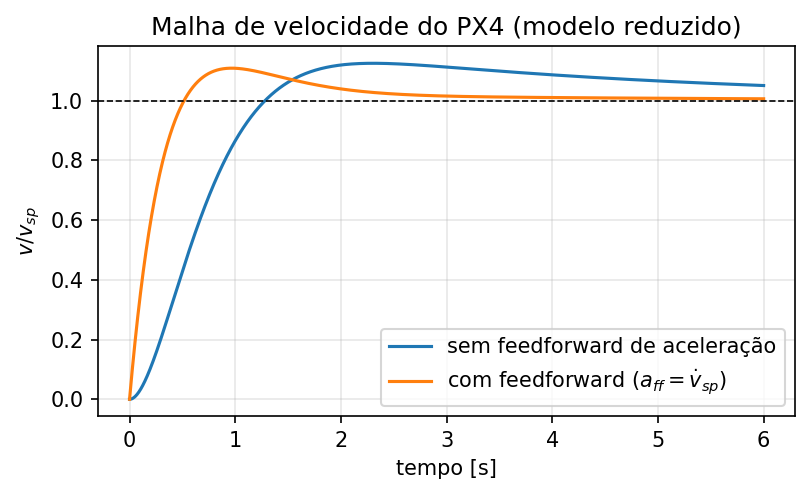
\includegraphics[width=0.75\textwidth]{px4_degrau.png}
\caption{Degrau de velocidade da PX4 pelo modelo \eqref{eq:tv}. Sem feedforward:
$t_{63\%}=\SI{0,70}{s}$, $M_p=12{,}5\%$, banda \SI{2,2}{rad/s}. Com feedforward:
$t_{63\%}=\SI{0,22}{s}$, $M_p=10{,}8\%$, banda \SI{5}{rad/s}.}
\label{fig:px4}
\end{figure}

\begin{atencao}
O \emph{feedforward} de aceleração mais que dobra a banda efetiva da malha interna.
Por isso todos os controladores publicam $\vect a$ junto com $\vect v$. O PID PBVS,
porém, gera $a_{ff}$ por diferença finita de velocidade
($(\vect v_k-\vect v_{ref})/\Ts$), o que amplifica ruído. Vale considerar filtrar ou
zerar esse termo se a medida for ruidosa.
\end{atencao}

\subsection{Identificação a partir de logs}
O modelo acima é uma aproximação. Para o TCC, \textbf{identifique} $T_v$ no Gazebo:
\begin{enumerate}
  \item Com o drone pairando em offboard, aplique degraus de velocidade (por exemplo,
        \SI{1}{m/s} em $x$ por \SI{3}{s}) publicando \code{/offboard/trajectory\_setpoint}.
  \item Grave \code{/fmu/out/vehicle\_local\_position\_v1} e o setpoint com
        \code{ros2 bag record}. Exporte para CSV.
  \item Rode \code{matlab/identificar\_px4.m}: ele estima um modelo de 1ª ordem com
        atraso ($K e^{-\theta s}/(\tau s+1)$) e um de 2ª ordem por \code{tfest}
        (System Identification Toolbox) ou, sem toolbox, por mínimos quadrados com
        \code{fminsearch}.
  \item Substitua $T_v(s)$ em \code{parametros.m} pelo modelo identificado.
\end{enumerate}

\section{Orçamento de atraso}
\begin{table}[H]
\centering
\begin{tabular}{@{}lr@{}}
\toprule
Fonte & Atraso médio \\
\midrule
Amostragem da câmera (\SI{30}{Hz}, meio período) & \SI{17}{ms} \\
Rastreador VitTrack + segmentação de profundidade & 30--\SI{60}{ms} \\
Pontes \code{ros\_gz\_bridge} / DDS & 2--\SI{10}{ms} \\
ZOH do controlador ($\Ts/2$) & \SI{25}{ms} \\
\midrule
\textbf{Total} & \textbf{$\approx$ 75--\SI{110}{ms}} \\
\bottomrule
\end{tabular}
\end{table}
No projeto, modele o atraso como $e^{-s\tau}$ (Padé: \code{pade(tau,2)}) no contínuo,
ou como $z^{-n}$ com $n=\lceil\tau/\Ts\rceil$ no discreto (\code{Lz.InputDelay = n}).
O estimador compensa em parte, porque extrapola a medida até o instante atual. A
extrapolação, porém, só é boa se a velocidade relativa estimada estiver certa
(\cref{cap:caso}).

\section{A planta vista pela malha externa}
\label{sec:planta-externa}
Juntando tudo, para um eixo e alvo parado:
\begin{align}
  \text{saída em aceleração (LQR, LQI, SMC, MPC, PN):}\quad
  & P_a(s) = \frac{T_v(s)}{s^2}\,e^{-s\tau}, \\
  \text{saída em velocidade (PID PBVS):}\quad
  & P_v(s) = \frac{T_v(s)}{s}\,e^{-s\tau}.
\end{align}

\paragraph{Detalhe importante: o amortecimento atua na referência.} Nos controladores
de aceleração, $e_v = v_{ref} - v_t$ usa a velocidade de \emph{referência}
$v_{ref} = u/s$, e não a velocidade medida. Com $u = -k_p e_p - k_d e_v$ e $v_t=0$:
\begin{equation}
  u = -k_p e_p - k_d\,\frac{u}{s}
  \;\Longrightarrow\;
  u = -\underbrace{\frac{k_p\,s}{s+k_d}}_{C_{eq}(s)}\,e_p ,
  \qquad
  L(s) = \frac{k_p\, s}{s+k_d}\cdot\frac{T_v(s)}{s^2}\,e^{-s\tau}.
  \label{eq:ceq}
\end{equation}
A única realimentação da dinâmica \emph{real} do drone é a posição medida (atrasada).
Esse é o motivo de a malha ser sensível ao atraso e à qualidade da estimativa.

\begin{table}[H]
\centering
\caption{Margens da malha externa com $T_v$ da \cref{tab:px4} (calculadas por
\code{matlab/analise\_margens.m}).}
\label{tab:margens}
\begin{tabular}{@{}lccccc@{}}
\toprule
Controlador & ganhos equivalentes & $\omega_c$ [rad/s] & PM ($\tau$=0) & PM ($\tau$=\SI{0,1}{s}) & margem de atraso \\
\midrule
LQR (yaml) & $k_p=4{,}09$, $k_d=3{,}39$ & 1,25 & \ang{57} & \ang{50} & \SI{0,70}{s} \\
MPC cinemático (yaml) & $k_p=2{,}16$, $k_d=2{,}06$ & 1,02 & \ang{55} & \ang{49} & \SI{0,83}{s} \\
PID PBVS (yaml) & $0{,}8/0{,}05/0{,}2$ & 0,87 & \ang{91} & \ang{86} & \SI{1,7}{s} \\
\bottomrule
\end{tabular}
\end{table}

\begin{figure}[H]
\centering
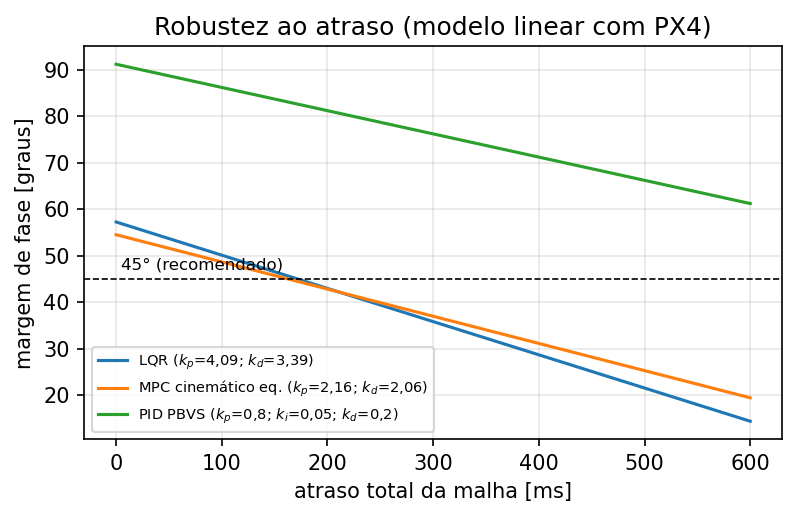
\includegraphics[width=0.75\textwidth]{margem_vs_atraso.png}
\caption{Margem de fase em função do atraso total. Com os ganhos atuais, todos ficam
acima de \ang{45} até $\approx\SI{150}{ms}$.}
\label{fig:margem-atraso}
\end{figure}

\begin{dica}
A \cref{tab:margens} mostra que, \emph{no modelo linear}, os ganhos do \code{yaml} têm
margem de sobra. Se a simulação oscila, a causa provável não está nos ganhos: está numa
não linearidade, numa saturação ou no estimador. Foi exatamente o que aconteceu no
\cref{cap:caso}. Faça sempre essa análise antes de ``baixar os ganhos''.
\end{dica}

\section{Saturações}
O nó aplica \code{applyLimits}: $|\vect a|\le$ \code{max\_acc} (taxa de variação de
$\vect v_{ref}$) e $|\vect v|\le$ \code{max\_vel}. Com saturação ativa, a malha deixa de
ser linear:
\begin{itemize}
  \item integradores (LQI, PID) acumulam erro: \emph{windup}. O código usa integração
        condicional (\code{integral\_zone}) e limita a norma de $\xi$;
  \item a análise por LGR vale só para pequenos erros. Grandes aproximações devem ser
        avaliadas em simulação;
  \item se o alvo for mais rápido que \code{max\_vel}, nenhum controlador alcança o
        standoff. Escolha cenários coerentes para a comparação.
\end{itemize}
